%
% $RCSfile: falsifying_polymorphism.tex,v $
%
% Copyright (C) 2002-2008. Christian Heller.
%
% Permission is granted to copy, distribute and/or modify this document
% under the terms of the GNU Free Documentation License, Version 1.1 or
% any later version published by the Free Software Foundation; with no
% Invariant Sections, with no Front-Cover Texts and with no Back-Cover
% Texts. A copy of the license is included in the section entitled
% "GNU Free Documentation License".
%
% http://www.cybop.net
% - Cybernetics Oriented Programming -
%
% http://www.resmedicinae.org
% - Information in Medicine -
%
% Version: $Revision: 1.1 $ $Date: 2008-08-19 20:41:06 $ $Author: christian $
% Authors: Christian Heller <christian.heller@tuxtax.de>
%

\subsubsection{Falsifying Polymorphism}
\label{falsifying_polymorphism_heading}
\index{Falsifying Polymorphism}
\index{Container Inheritance}
\index{Hashtable}
\index{Copy Constructor}

Problems can occur when inheriting containers. This is now demonstrated on a Java
example adopted from \cite{javaiaq}.

\begin{figure}[ht]
    \begin{center}
        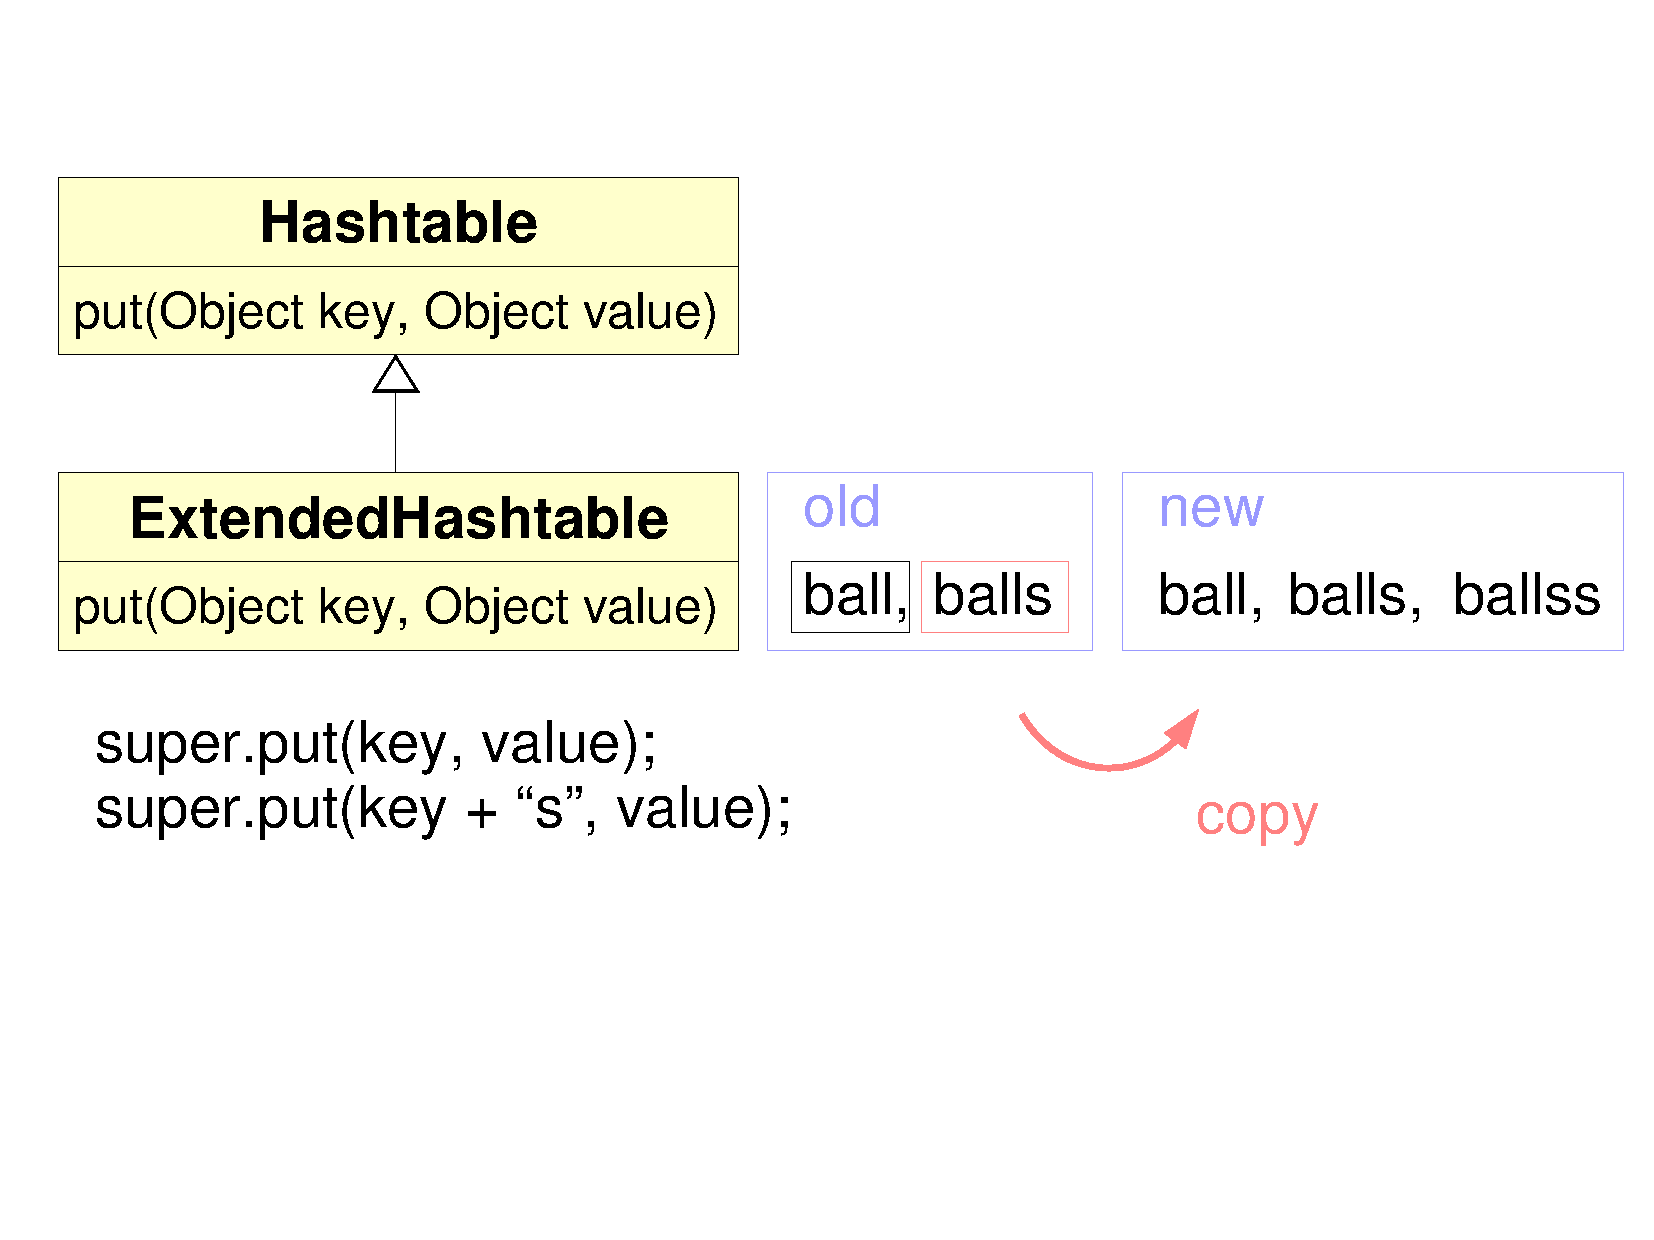
\includegraphics[scale=0.3,angle=-90]{graphic/falsifying.pdf}
        \caption{Falsified Contents with Container Inheritance}
        \label{falsifying_figure}
    \end{center}
\end{figure}

A class \emph{ExtendedHashtable} extends the standard container \emph{Hashtable}
(figure \ref{falsifying_figure}). The \emph{ExtendedHashtable} overrides the
\emph{put} method and lets it do two calls to the \emph{put} method of the
superior class \emph{Hashtable}, the second of these calls adding the letter
\emph{s} to the key.

A first object of type \emph{ExtendedHashtable} gets filled by calling the
\emph{put} method which adds two identical element values with the two different
keys \emph{ball} and \emph{balls} to the container. When the container is full,
a new one with extended size gets created and all values of the old have to be
copied into the new container, which is again of type \emph{ExtendedHashtable}.

If the \emph{put} method is now used to accomplish this, a falsified container
with more elements than the original one will be retrieved. The copying of the
first element \emph{ball} results in two elements \emph{ball} and \emph{balls},
placed in the new container. The copying of the second element \emph{balls} adds
two further elements \emph{balls} and \emph{ballss}, whereby the \emph{balls}
key stemming from the copying of the first element gets overwritten.

This example demonstrates only the principle of how the automatic size
extension of inherited container objects with element copying using
container-owned methods can incorrectly modify the container contents. The Java
language's \emph{Hashtable} class uses a slightly different mechanism, handing
over the hashtable object as parameter of a copy constructor which internally
calls a \emph{putAll} method which finally calls the \emph{put} method. Other
OOP languages may use different mechanisms. Of course, there are workarounds to
avoid the described troubles. But as a matter of fact, container inheritance
may -- due to polymorphism -- cause unpredictable behaviour leading to
\emph{falsified} container contents.

The language and interpreter introduced in chapters
\ref{cybernetics_oriented_language_heading} and
\ref{cybernetics_oriented_interpreter_heading} base on just one container
structure for knowledge representation, that covers many of the traditional
forms of containers.
